\documentclass[tikz]{standalone}
\usepackage{tikz}
\usepackage[AutoFakeBold=true,AutoFakeSlant=true]{xeCJK}
\usepackage[zihao=-4,UTF8,heading=true]{ctex}
\usepackage[simplified]{pgf-umlcd}
\usetikzlibrary{fit} %形状
\usetikzlibrary{positioning} %不加方向运算可能出错
\usetikzlibrary{arrows.meta} %箭头
\usetikzlibrary{calc}

\setCJKmainfont{微软雅黑}
\begin{document}
	\thispagestyle{empty}
    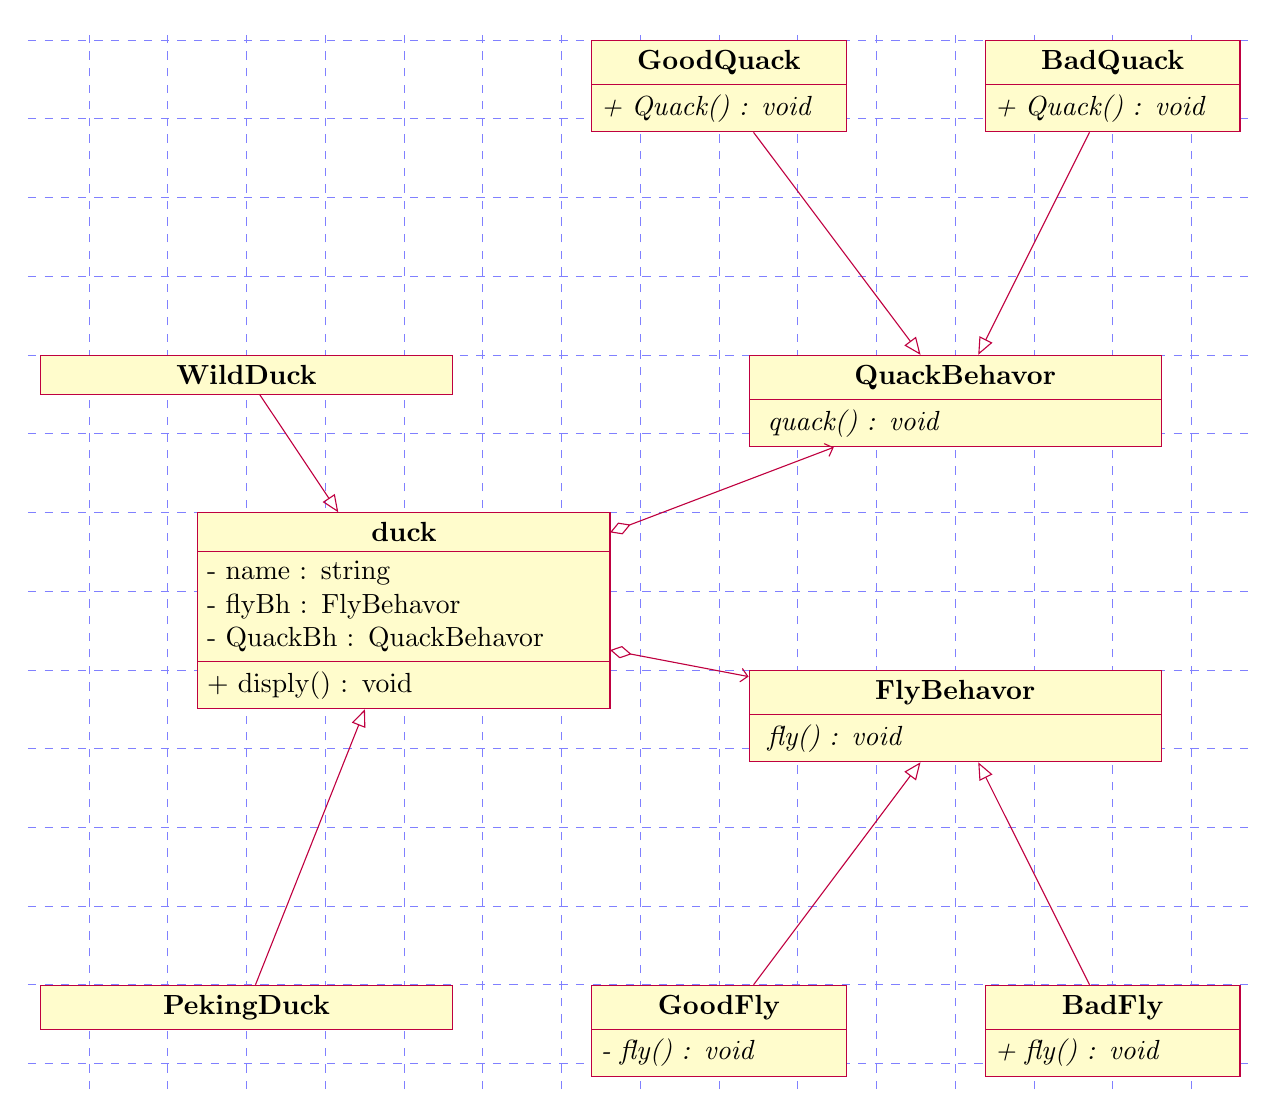
\begin{tikzpicture}[show background grid]
        \begin{class}[]{FlyBehavor}{6, -2}
            \operation[0]{ fly() : void}
        \end{class}
        \begin{class}[]{QuackBehavor}{6,2}
            \operation[0]{ quack() : void}
        \end{class}
        
        \begin{class}[text width=5cm]{duck}{-1,0}
            \attribute{- name : string }
            \attribute{- flyBh : FlyBehavor }
            \attribute{- QuackBh : QuackBehavor }
            \operation{+ disply() : void}
        \end{class}
        \begin{class}[]{WildDuck}{-3, 2}
            \inherit{duck}
        \end{class}
        \begin{class}[]{PekingDuck}{-3, -6}
            \inherit{duck}
        \end{class}
        \aggregation{duck}{}{}{QuackBehavor}
        \aggregation{duck}{}{}{FlyBehavor}
        \begin{class}[text width = 3cm]{GoodFly}{3,-6}
            \operation[0]{- fly() : void}
            \inherit{FlyBehavor}
        \end{class}
        \begin{class}[text width = 3cm]{BadFly}{8,-6}
            \operation[0]{+ fly() : void}
            \inherit{FlyBehavor}
        \end{class}
        \begin{class}[text width = 3cm]{GoodQuack}{3,6}
            \operation[0]{+ Quack() : void}
            \inherit{QuackBehavor}
        \end{class}
        \begin{class}[text width = 3cm]{BadQuack}{8,6}
            \operation[0]{+ Quack() : void}
            \inherit{QuackBehavor}
        \end{class}
        
    \end{tikzpicture}

\end{document}